%-------------------------------------------------
%	Version: 0.0
%	fecha de entrega
%
%-------------------------------------------------

\documentclass[11pt]{report}

%packages
\usepackage{graphicx}
\usepackage{subcaption}

\usepackage[utf8]{inputenc}
\usepackage[spanish, es-nodecimaldot]{babel}
\usepackage{setspace}
\usepackage{ragged2e}

\usepackage{amsmath}
\usepackage{amsthm}
\usepackage{amssymb}
\usepackage{mathtools}
\usepackage{siunitx}
\usepackage[thinc]{esdiff} %derivadas faciles
\usepackage{physics} %algunos simbolos de derivadas

%path donde se encuentran las imagenes
\graphicspath{ {./figuras/} }

%---------------------------------------------------------------
%ABREVIACIONES DE COMANDOS

\theoremstyle{plain}
\newtheorem{thm}{Teorema}[chapter] % reset theorem numbering for each chapter

\theoremstyle{definition}
\newtheorem{defn}[thm]{Definición} % definition numbers are dependent on theorem numbers
\newtheorem{exmp}[thm]{Ejemplo} % same for example numbers

\newcommand{\chaptercontent}{
\section{Basics}
\begin{defn}Here is a new definition.\end{defn}
\begin{thm}Here is a new theorem.\end{thm}
\begin{thm}Here is a new theorem.\end{thm}
\begin{exmp}Here is a good example.\end{exmp}
\subsection{Some tips}
\begin{defn}Here is a new definition.\end{defn}
\section{Advanced stuff}
\begin{defn}Here is a new definition.\end{defn}
\subsection{Warnings}
\begin{defn}Here is a new definition.\end{defn}
}

\usepackage{biblatex}
%\addbibresource{Tarea1.bib}

\begin{document}

\begin{titlepage}
\title{Titulo_del_trabajo}

%-------------------------------------------------
%PORTADA
%-------------------------------------------------

	\centering
	{\scshape\LARGE Universidad Autónoma de Yucatán  \\ Facultad de ingeniería\par}
	\vspace{1cm}
	{\scshape\Large Instrumentación\par}
	\vspace{1.5cm}
	{\huge\bfseries Apuntes de clase\par}
	\vspace{0.7cm}
	{\begin{figure}[!h]
	\centering
    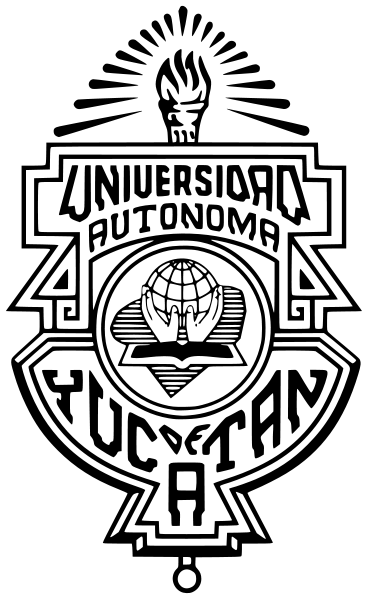
\includegraphics[scale=0.3]{UADY.png}
	\end{figure}}
	\vspace{0.7cm}
	{\Large\itshape Erick Al. Casanova Cortés\par}
	{\Large\itshape Matricula: 15014866 \par}
	\vfill
	{\scshape\Large Docente\par
	Mto. Renan Quijano\par}
	\vfill
	{\Large{\bfseries Fecha de modificación:\today} }

	\vfill
	
\end{titlepage}

%-------------------------------------------------
%Inicio del documento
%-------------------------------------------------

\tableofcontents

%-------------------------------------------------
% Introducción
%-------------------------------------------------
\chapter{Introducción}

Horarios de asesorías, Lunes, miércoles y jueves de 10:00 - 17:00hrs \\

El curso se dará de manera virtual y el contenido estará en la plataforma del la escuela, así como la comunicación será por el correo de la escuela.\\

\section{Formativa}

Tareas: 10\% \\
Prácticas: 40\% \\
Proyecto final: 50\% \\

Todas las actividades se realizarán en el horario de clase:

\section{Objetivo del curso}
Aprender acerca de los métodos y las herramientas actuales que permitan instrumentar sistemas para el control y automatización de procesos

\section{Metas}
Conocer los instrumentos de medición y el equipo electrónico moderno utilizados para la instrumentación de procesos.
Aprender las técnicas modernas de instrumentación
Conocer los procesos de caracterización de los sensores
Diseño de sistemas básicos basados en microcontroladores
ver tendencias 


\section{Software de apoyo}
Simulador de circuitos y electrónicos.\\
API para programación de microcontroladores.\\
Software para análisis estadístico de datos.\\
Software para instrumentación virtual.


\section{Formato adas}
Archivo PDF con nombre: CasanovaE8MTarea\#.pdf \\
Portada \\
Descripción de la actividad \\
Contenido \\
Ortografía y redacción\\

%-------------------------------------------------
% Fundamentos de mediciones
%-------------------------------------------------

\chapter{Fundamentos de mediciones}

%-------------------------------------------------
%Clasificación y conceptos básicos de los instrumentos
\section{Clasificación y conceptos básicos de los instrumentos}

Antes se utilizaba partes del cuerpo para medir, ya que era necesario llevar una cuenta o un registro de las cantidades.

Actualmente se necesita monitorear diferentes procesos para este propósito se recurre a la instrumentación.
Es común el empleo de sistema de medición para el registro de variables, en vez de instrumentos de medición individuales.
El sistema de medición puede dividirse en diferentes componentes.

El sistema de medición se compone de:
\begin{enumerate}
	\item variable física
	\item sensor primario
	\item conversión de variable (circuito)
	\item acondicionamiento de señal (amplificador)
	\item salida
\end{enumerate}

En la instrumentación nos interesa tomar algo del entorno, y se entrega una salida después de un procesamiento. Este tipo de salidas debe estar estandarizadas, lo que quiere decir que están normados para tener elementos compatibles, lo que nos permitiría agregar nuevos sensores sobre el mismo rango.

recordad que los estándares de medición se miden en el SI

\section{Simbología y normatividad}

Criterios para la selección de instrumentos
Error asociado a los instrumentos de medición

\section{Principal criterios para la selección de instrumentos}

\subsection*{Respuesta de primer orden}
Los instrumentos con respuesta de primer orden se caracterizan por una constante de tiempo $\tau$.
Si el mesurado sufre un cambio abrupto en $\Delta$, tau es el tiempo que toma a $\Delta$ en cambiar aprox $63\%$

\subsection*{Respuesta de segundo orden}
La respuesta de un instrumento de segundo orden es idéntica al comportamiento de un sistema armónico amortiguado simple.
La mayoría de los instrumentos son críticamente amortiguados, es decir, su salida permaneces dentro de un porcentaje determinado del valor final, que es alcanzado en un corto tiempo.

\subsection*{Calibración}
Los instrumentos sólo pueden ajustarse a las características estáticas y dinámicas si están debidamente calibrados. Esto se realiza normalmente de modo jerárquico, calibrando cada instrumento contra otro instrumento similar aún más exacto, cuyo único propósito es calibrar otros instrumentos.

\subsection*{Trazabilidad}
Para la calibración, debe ser posible comprobar una cadena ininterrumpida de comparaciones que termina en algún organismo de estandarización nacional.

\subsection*{Procesamiento de señal}
El procesamiento de las señales provenientes de instrumentos de medición se utiliza para mejorar la calidad de la lectura de la señal a la salida del sistema de mediciones o para extraer información util.

\subsection*{Incertidumbre de las mediciones}
Normalmente son dos

\begin{enumerate}
	\item incertidumbre aleatoria
	\item sistematica
\end{enumerate}

La aleatoria es por fluctuaciones o ruido de la señal, normalmente son cuando las mediciones son humanas (se observa el resultado).
Las sistemáticas no se pueden corregir mediante el promedio de mediciones repetidas, el error humano está involucrado en los error sistemáticos

%-------------------------------------------------
% Métodos instrumentales de análisis
%-------------------------------------------------

\chapter{Métodos instrumentales de análisis}

Instrumentación moderna
Adquisición de datos


%-------------------------------------------------
% Aplicaciones de los microcontroladores en 
% sistemas de instrumentación
%-------------------------------------------------

\chapter{Aplicaciones de los microcontroladores en sistemas de instrumentación}

Adquisición de dados a traves de microcontroladores
Procesamiento y análisis de variables físicas...


%-------------------------------------------------
% Técnicas modernas para automatización de procesos
%-------------------------------------------------

\chapter{Técnicas modernas para automatización de procesos}
Dispositivos reconfigurables
Niveles de integración de los componentes electrónicos
Acondicionadores de señales monolíticos
Controladores analógicos integrados
Transmisión de datos a la web
Instrumentación





%-------------------------------------------------
%Final del documento
%-------------------------------------------------

\end{document}
